\documentclass[12pt,a4paper]{article}

% Encoding & language
\usepackage[utf8]{inputenc}
\usepackage[T1]{fontenc}
\usepackage[main=english]{babel}
\usepackage{caption}
\usepackage{booktabs}

% untuk kode
\usepackage{listings}

% Margin & spacing
\usepackage{geometry}
\geometry{margin=1in}
\usepackage{setspace}
\setstretch{1.2}

% Math & extras
\usepackage{enumitem}
\usepackage{amsmath,amssymb,amsthm}
\usepackage{algorithm}
\usepackage{algpseudocode}

\theoremstyle{remark}
\newtheorem*{solusi}{Solusi}

% Paket untuk gambar
\usepackage{graphicx}
\usepackage{tikz}
\usetikzlibrary{shapes.geometric, arrows, positioning}

% Etc
\usepackage{titling}
\usepackage{csquotes}
\usepackage{subcaption}
% Untuk hyperlink
\usepackage{hyperref}

% --- Biblatex dengan IEEE style ---
\usepackage[backend=biber,style=ieee,language=english]{biblatex}
\addbibresource{refs.bib}

\DefineBibliographyStrings{english}{%
  references   = {Daftar Pustaka},
  bibliography = {Daftar Pustaka},
  and          = {dan},
  andothers    = {dkk.},
  pages        = {hlm.},
}

% STYLING
\setlength{\parindent}{2em}

% OVERRIDE Caption
\captionsetup[figure]{labelfont=bf, name=Gambar, justification=centering}
\captionsetup[table]{labelfont=bf, name=Tabel, justification=centering}



% --- Title page ---
\title{%
  \textbf{Tugas Mata Kuliah} \\
  \large Rekayasa Fitur dan Pengenalan Pola (RFPP) \\
  \large Klasifikasi Melanoma dengan Pendekatan \textit{Hand-crafted Features} \\ dan Pemelajaran Mesin}
  
\author{Khalilullah Al Faath \\ NIU: 566643 \\ Magister Ilmu Komputer \\ [1cm]
  \includegraphics[width=0.4\textwidth]{images/logo-ugm.png}}
\date{Universitas Gadjah Mada \\ Semester Gasal 2025/2026}

\makeatletter
\renewcommand{\maketitle}{%
  \begin{titlepage}
    \centering
    \vspace*{2cm}
    
    {\LARGE \@title \par}
    \vspace{2cm}
    
    {\large \@author \par}
    
    \vfill
    
    {\large \@date \par}
  \end{titlepage}
}
\makeatother

\begin{document}

\maketitle
\thispagestyle{empty}

% Daftar isi dan daftar gambar/tabel

% override label
\renewcommand{\contentsname}{Daftar Isi}
\renewcommand{\listfigurename}{Daftar Gambar}
\renewcommand{\listtablename}{Daftar Tabel}

% daftar isi
\tableofcontents

\newpage

% daftar gambar
\listoffigures

\newpage

% daftar tabel
\listoftables

\newpage
\setcounter{page}{1}

\section{Pendahuluan}
Melanoma maligna merupakan bentuk neoplasma kulit yang paling mematikan yang merupakan hasil transformasi melanosit, yaitu sel yang berasal dari \textit{neural crest}. Karena asal-usul embriologisnya, melanoma tidak hanya terbatas pada kulit, tetapi juga dapat berkembang di lokasi lain tempat sel \textit{neural crest} bermigrasi, seperti traktus gastrointestinal, otak, dan mata (melanoma okular). Secara patofisiologis, perkembangan melanoma sangat dipengaruhi oleh faktor lingkungan (terutama paparan radiasi UV), genetik (seperti mutasi pada gen BRAF, CDKN2A, CDK4), dan imunologis \cite{heistein_malignant_2025}.

Urgensi pengembangan sistem deteksi dan klasifikasi melanoma didasari oleh tren peningkatan insiden dan risiko fatalitas yang yang tinggi. Berdasarkan data \textit{National Cancer Instite (NCI) Surveillance, Epidemiology, and End Results (SEER)}, (1) melanoma kini  merupakan kanker ganas yang paling umum yang terjadi di pria dan wanita, (2) pada tahun 2023, diperkirakan terdapat 97.000 kasus baru di Amerika Serikat dengan estimasi 7.990 kematian \cite{siegel_cancer_2023}, (3) Tingkat kelangsungan hidup relatif 5 tahun (5-year relative survival rate) sangat bergantung pada stadium saat diagnosis: pasien dengan melanoma stadium 0 (in-situ) memiliki tingkat kelangsungan hidup mencapai 97\% hingga 100\%. Sebaliknya, angka ini menurun drastis menjadi sekitar 30\% hingga 52\% bagi pasien yang terdiagnosis pada stadium IV (metastatik) \cite{heistein_malignant_2025}, (4) di Indonesia, pada tahun 2020, angka kasus kanker kulit mencapai 18.000 kasus dengan angka kematian sekitar 3.000 \cite{primaya_hospital_editor_kanker_2023}.

Deteksi dini melanoma dapat dilakukan dengan menggunakan metode jembatan keledai "ABCDE", yaitu "A" untuk \textit{Asymmetry} atau asimetris, "B" untuk \textit{Border} atau tepi, "C" untuk \textit{color} atau warna, "D" untuk \textit{Diameter}, dan "E" untuk \textit{Evolving} atau berevolusi \cite{heistein_malignant_2025}. Gambar~\ref{fig:abcde} menggambarkan karakteristik khusus dari melanoma.

\begin{figure}[H]
  \centering
  \includegraphics[width=0.75\linewidth]{images/abcde-melanoma.png}
  \caption{Karakteristik Melanoma}
  \label{fig:abcde}
\end{figure}

Pengembangan sistem \textit{Computer-Aided Diagnosis (CAD)} untuk deteksi melanoma telah menjadi fokus penelitian intensif dalam beberapa dekade terakhir. Secara garis besar, penelitian-penelitian sebelumnya dapat dikelompokkan menjadi dua pendekatan utama: metode berbasis ekstraksi fitur manual atau (\textit{hand-crafted features}) dan metode berbasis pemelajaran dalam atau \textit{Deep Learning}.

\begin{description}
  \item[Pendekatan ekstraksi manual] Pendekatan pertama, yaitu metode ekstraksi fitur manual, berfokus pada pemodelan karakteristik visual melanoma berdasarkan pengetahuan klinis dan aturan morfologi. Pada pendekatan ini, proses analisis citra dilakukan melalui tahapan pra-pemrosesan, segmentasi lesi, dan ekstraksi fitur berbasis ciri geometris, tekstur, atau warna. Contohnya termasuk penggunaan fitur statistik orde pertama, \textit{Histogram of Oriented Gradients (HOG)}, \textit{Local Binary Patterns (LBP)}, momen bentuk, hingga parameter geometrik seperti asimetri, \textit{compactness}, dan \textit{eccentricity}. Pendekatan ini memiliki keunggulan berupa interpretabilitas yang tinggi karena parameter yang dianalisis selaras dengan kriteria klinis seperti aturan ABCDE. Namun, performanya sangat bergantung pada kualitas segmentasi dan sensitivitas model terhadap variasi perangkat fotografi, pencahayaan, serta keberadaan artefak seperti rambut, bayangan, dan variasi kulit \cite{tumpa_artificial_2021, mahum_skin_2022, almaraz-damian_melanoma_2020}.
  \item[Pendekatan pemelajaran dalam] Sebaliknya, pendekatan berbasis pemelajaran dalam (\textit{Deep Learning}) memanfaatkan jaringan saraf tiruan berlapis banyak, khususnya \textit{Convolutional Neural Network} (CNN), untuk mengekstraksi representasi fitur secara otomatis tanpa memerlukan desain fitur manual oleh pakar. Model seperti ResNet, EfficientNet, dan Vision Transformer (ViT) telah menunjukkan performa unggul dalam kompetisi internasional seperti International Skin Imaging Collaboration (ISIC). Keunggulan utama pendekatan ini adalah kemampuannya untuk belajar dari data berskala besar, mengurangi ketergantungan pada pra-pemrosesan, serta meningkatkan robustnes terhadap variasi pola, warna, dan tekstur lesi kulit. Namun, tantangannya mencakup kebutuhan dataset besar yang teranotasi dengan baik, risiko bias algoritmik akibat ketidakseimbangan distribusi data (misalnya warna kulit pasien), serta keterbatasan interpretabilitas (\textit{black-box problem}) \cite{esteva_dermatologist-level_2017,li_skin_2017, wu_skin_2022}.
\end{description}

Klasifikasi melanoma yang dilakukan pada tugas ini dilakukan dengan menggunakan ekstraksi fitur manual dengan model pemelajaran mesin \textit{Support Vector Machine} (SVM).

\section{Metode}
Bagian ini menjelaskan alur langkah yang dilakukan pada tugas ini. Gambar~\ref{fig:diagramalir} menunjukkan alur langkah metode yang diusulkan.

\begin{figure}[H]
  \centering
  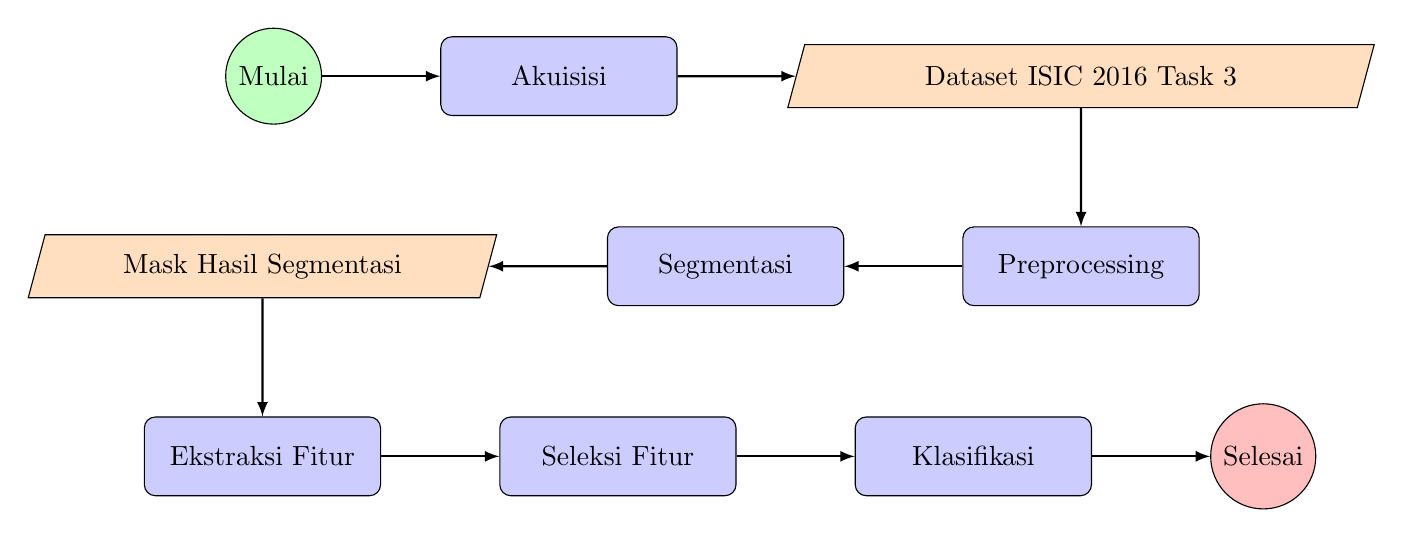
\begin{tikzpicture}[
      node distance=15mm,
      proc/.style={
          rectangle,
          draw,
          rounded corners,
          align=center,
          minimum width=30mm,
          minimum height=10mm,
          fill=blue!20
        },
      io/.style={
          trapezium,
          trapezium left angle=75,
          trapezium right angle=105,
          draw,
          align=center,
          minimum width=25mm,
          minimum height=8mm,
          fill=orange!25
        },
      term-start/.style={
          circle,
          draw,
          align=center,
          minimum size=10mm,
          fill=green!25
        },
      term-finish/.style={
          circle,
          draw,
          align=center,
          minimum size=10mm,
          fill=red!25
        },
      arrow/.style={
          -latex,
          thick
        }
    ]

    % Nodes
    \node[term-start] (mulai) {Mulai};
    \node[proc, right=of mulai] (akuisisi) {Akuisisi};
    \node[io, right=of akuisisi] (isic) {Dataset ISIC 2016 Task 3};
    \node[proc, below=of isic] (pre) {Preprocessing};
    \node[proc, left=of pre] (seg) {Segmentasi};
    \node[io, left=of seg] (mask) {Mask Hasil Segmentasi};
    \node[proc, below=of mask] (ekstrak) {Ekstraksi Fitur};
    \node[proc, right=of ekstrak] (seleksi) {Seleksi Fitur};
    \node[proc, right=of seleksi] (klasif) {Klasifikasi};
    \node[term-finish, right=of klasif] (selesai) {Selesai};

    % Arrows
    \draw[arrow] (mulai) -- (akuisisi);
    \draw[arrow] (akuisisi) -- (isic);
    \draw[arrow] (isic) -- (pre);
    \draw[arrow] (pre) -- (seg);
    \draw[arrow] (seg) -- (mask);
    \draw[arrow] (mask) -- (ekstrak);
    \draw[arrow] (ekstrak) -- (seleksi);
    \draw[arrow] (seleksi) -- (klasif);
    \draw[arrow] (klasif) -- (selesai);

  \end{tikzpicture}
  \caption{Diagram alir metode yang dilakukan}
  \label{fig:diagramalir}
\end{figure}





\subsection{Akuisisi}
Dataset yang digunakan pada tugas ini adalah Dataset ISIC 2016 Task 3. \footnote{Dataset ini dapat diunduh di pranala berikut \url{https://challenge.isic-archive.com/landing/2016/39/}} Dataset ini merupakan himpunan citra dermoskopik yang digunakan untuk menyelesaikan permasalahan klasifikasi lesi kulit menjadi dua kategori, yaitu \textit{benign} (non-malignant) dan \textit{malignant}. Gambar~\ref{fig:contoh-data} menunjukkan contoh data yang ada pada Dataset, sementara Gambar~\ref{fig:contoh-benign} menunjukkan contoh citra berlabel \textit{benign} dan \textit{malignant}.

\begin{figure}[H]
  \centering
  \includegraphics[trim=0 5cm 0 3cm, clip, width=1\textwidth]{images/contoh-data.pdf}
  \caption{Contoh citra yang ada pada Dataset ISIC 2016 Task 3.}
  \label{fig:contoh-data}
\end{figure}

\begin{figure}[H]
  \centering
  \includegraphics[trim=0 5cm 0 3cm, clip, width=1\textwidth]{images/contoh-benign.pdf}
  \caption{Contoh citra \textit{benign} dan \textit{malignant}.}
  \label{fig:contoh-benign}
\end{figure}

Dataset pelatihan terdiri atas 900 citra lesi kulit dalam format JPEG dengan resolusi bervariasi. Setiap citra dinamai menggunakan pola \texttt{ISIC\_<image\_id>.jpg} dengan tujuh digit pengenal unik. Berkas pelatihan dilengkapi dengan \textit{Training Ground Truth} berupa sebuah berkas CSV yang memuat dua kolom: (1) \texttt{image\_id} yang sesuai dengan nama berkas citra, dan (2) label diagnosis definitif (\textit{benign} atau \textit{malignant}) yang ditentukan berdasarkan konsensus pakar serta laporan patologi.

Selain itu, disediakan pula seperangkat \textit{Test Data} yang terdiri dari 379 citra dengan format yang sama. Berbeda dengan data pelatihan, data uji tidak disertai label kebenaran untuk menjaga objektivitas evaluasi. Pada proses kompetisi aslinya, peserta diminta mengunggah hasil prediksi dalam format CSV dua kolom berisi \texttt{image\_id} dan skor probabilistik dalam rentang [0.0, 1.0], dengan nilai di atas 0.5 mengindikasikan prediksi \textit{malignant} \cite{isic_committee_isic_2016}.

Dapat dilihat pada Gambar~\ref{fig:contoh-data} terdapat beberapa jenis \textit{noice} yang dapat diidentifikasi, yaitu \textit{border noice}, \textit{hair noice}, dan \textit{object noice}.

\subsection{\textit{Pre-processing}}
Setelah mendapatkan Dataset, dilakukan \textit{pre-processing} atau pra-pemrosesan untuk menghilangkan sebagian noice. Gambar~\ref{fig:preprocessing} menunjukkan langkah-langkah pra-pemrosesan yang dilakukan.

\begin{figure}[H]
  \centering
  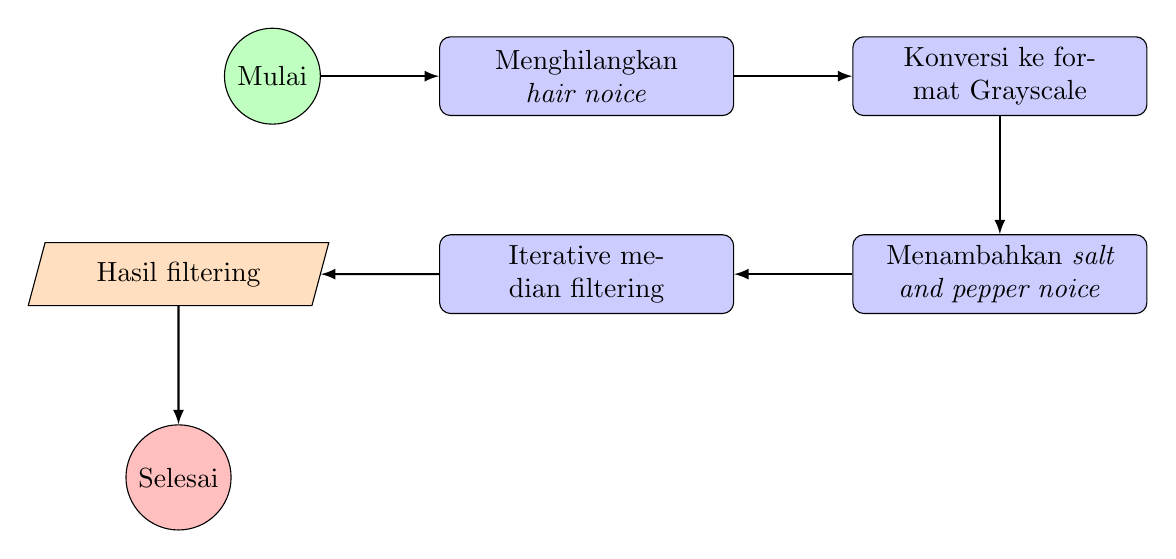
\begin{tikzpicture}[
      node distance=15mm,
      proc/.style={
          rectangle,
          draw,
          rounded corners,
          align=center,
          minimum width=30mm,
          minimum height=10mm,
          text width=35mm,
          fill=blue!20
        },
      io/.style={
          trapezium,
          trapezium left angle=75,
          trapezium right angle=105,
          draw,
          align=center,
          minimum width=25mm,
          minimum height=8mm,
          fill=orange!25
        },
      term-start/.style={
          circle,
          draw,
          align=center,
          minimum size=10mm,
          fill=green!25
        },
      term-finish/.style={
          circle,
          draw,
          align=center,
          minimum size=10mm,
          fill=red!25
        },
      arrow/.style={
          -latex,
          thick
        }
    ]

    % Nodes
    \node[term-start] (mulai) {Mulai};
    \node[proc, right=of mulai] (hair) {Menghilangkan \textit{hair noice}};
    \node[proc, right=of hair] (konversi) {Konversi ke format Grayscale};
    \node[proc, below=of konversi] (salt) {Menambahkan \textit{salt and pepper noice}};
    \node[proc, left=of salt] (filter) {Iterative median filtering};
    \node[io, left=of filter] (hasil) {Hasil filtering};
    \node[term-finish, below=of hasil] (selesai) {Selesai};

    % Arrows
    \draw[arrow] (mulai) -- (hair);
    \draw[arrow] (hair) -- (konversi);
    \draw[arrow] (konversi) -- (salt);
    \draw[arrow] (salt) -- (filter);
    \draw[arrow] (filter) -- (hasil);
    \draw[arrow] (hasil) -- (selesai);

  \end{tikzpicture}



  \caption{Diagram alir pra-pemrosesan.}
  \label{fig:preprocessing}
\end{figure}

Setiap tahap pra-pemrosesan memiliki tujuan spesifik untuk mempersiapkan citra sebelum dilakukan segmentasi dengan mengikuti alur dari penelitian \textcite{jaseema_yasmin_improved_2012}.

\begin{enumerate}
  \item \textbf{Menghilangkan \textit{hair noise}}: Pada citra dermoskopik, rambut yang menutupi lesi dapat mengganggu analisis dan segmentasi. Oleh karena itu, rambut dihilangkan menggunakan operasi morfologi \textit{black-hat} yang diikuti dengan \textit{inpainting} untuk menutupi area rambut dengan piksel sekitarnya, sehingga citra menjadi lebih bersih.

  \item \textbf{Konversi ke format Grayscale}: Citra RGB dikonversi menjadi citra intensitas (grayscale) untuk menyederhanakan data dan mengurangi kompleksitas komputasi. Dengan ini, analisis selanjutnya hanya fokus pada intensitas piksel, sehingga pengaruh variasi warna yang tidak relevan dapat diminimalkan.

  \item \textbf{Menambahkan \textit{salt and pepper noise}}: Tahap ini dilakukan untuk menyiapkan citra dalam kondisi yang memungkinkan pengujian ketahanan metode filter. Noise buatan ditambahkan pada citra grayscale agar metode \textit{iterative median filtering} dapat diuji efektivitasnya dalam menghilangkan noise dan mempertahankan tepi lesi.

  \item \textbf{Iterative Median Filtering}: Citra yang telah diberi noise kemudian difilter menggunakan metode median secara iteratif. Filter median efektif untuk menghilangkan noise impulsif (\textit{salt and pepper}) tanpa merusak kontur objek penting. Proses iteratif memastikan noise tersisa dapat dihilangkan secara bertahap, sambil mempertahankan detail lesi.

  \item \textbf{Hasil Filtering}: Tahap ini menghasilkan citra yang bersih dari noise, dengan kontur lesi tetap terjaga. Citra hasil ini siap digunakan untuk tahap segmentasi dan ekstraksi fitur selanjutnya.
\end{enumerate}

Gambar~\ref{fig:hasil-preprocessing} memperlihatkan contoh hasil tiap tahap filtering pada citra dermoskopik.

\begin{figure}[H]
  \centering
  \includegraphics[trim=0 5cm 0 3cm, clip, width=1\textwidth]{images/hasil-filtering.pdf}
  \caption{(1) Konversi ke Grayscale; (2) Menambahkan \textit{salt and pepper noice}; (3) Menerapkan \textit{Iterative median filtering}}
  \label{fig:hasil-preprocessing}
\end{figure}


% \begin{figure}[H]
%     \centering
%     \includegraphics[width=1\linewidth]{images/diagram alir.pdf}
%     \caption{Diagram alir metode yang diusulkan.}
%     \label{fig:diagramalir}
% \end{figure}


% \begin{table}[H]
%     \centering
%     \begin{tabular}{c|c|c}
%         No. & Kelas & Jumlah data \\
%         1 & Maju & 22 \\
%         2 & Mundur & 26 \\
%         3 & Berhenti & 23 \\
%         4 & Kiri & 25 \\
%         5 & Kanan & 26 \\
%     \end{tabular}
%     \caption{Banyaknya data tiap kelas.}
%     \label{tab:rincianjumlahdata}
% \end{table}



\section{Hasil dan Pembahasan}

\subsection{Dataset yang digunakan}

\subsection{Lingkungan pengujian}

\subsection{Hasil}

\subsection{Diskusi}

\section{Kesimpulan}

Berdasarkan hasil dan analisis yang telah dilakukan, dapat disimpulkan bahwa:

Kode tersedia pada \textit{repository} GitHub \url{https://github.com/khalilullahalfaath/RFPP---Melanoma-Classification-Handcrafted-Features-}.

\newpage

% Daftar pustaka
\printbibliography

\end{document}
